\chapter{Web reasoning}


\section{Semantic web}

\begin{description}
    \item[Semantic web] \marginnote{Semantic web}
        Method to represent and reason on the data available on the web.
        Semantic web aims to preserve the characteristics of the web, this includes:
        \begin{itemize}
            \item Globality.
            \item Information distribution.
            \item Information inconsistency of contents and links (as everyone can publish).
            \item Information incompleteness of contents and links.
        \end{itemize}

        Information is structured using ontologies and logic is used as inference mechanism.
        New knowledge can be derived through proofs.

    \item[Uniform resource identifier] \marginnote{URI}
        Naming system to uniquely identify concepts.
        Each URI corresponds to one and only one concept, but multiple URIs can refer to the same concept.

    \item[XML] \marginnote{XML}
        Markup language to represent hierarchically structured data.
        An XML can contain in its preamble the description of the grammar used within the document.

    \item[Resource description framework (RDF)] \marginnote{Resource description framework (RDF)}
        XML-based language to represent knowledge.
        Based on triplets:
        \begin{center}
            \texttt{<subject, predicate, object>}\\
            \texttt{<resource, attribute, value>}
        \end{center}

        RDF supports:
        \begin{descriptionlist}
            \item[Types] Using the attribute \texttt{type} which can assume an URI as value. 
            \item[Collections] Subjects and objects can be bags, sequences or alternatives.
            \item[Meta-sentences] Reification of the sentences (e.g. "X says that Y\dots").
        \end{descriptionlist}

        \begin{description}
            \item[RDF schema] \marginnote{RDF schema}
                RDF can be used to describe classes and relations with other classes (e.g. \texttt{type}, \texttt{subClassOf}, \texttt{subPropertyOf}, \dots)
            
            \item[Representation] \phantom{}
                \begin{descriptionlist}
                    \item[Graph] A graph where nodes are subjects or objects and edges are predicates.
                        \begin{example} \phantom{}
                            \begin{center}
                                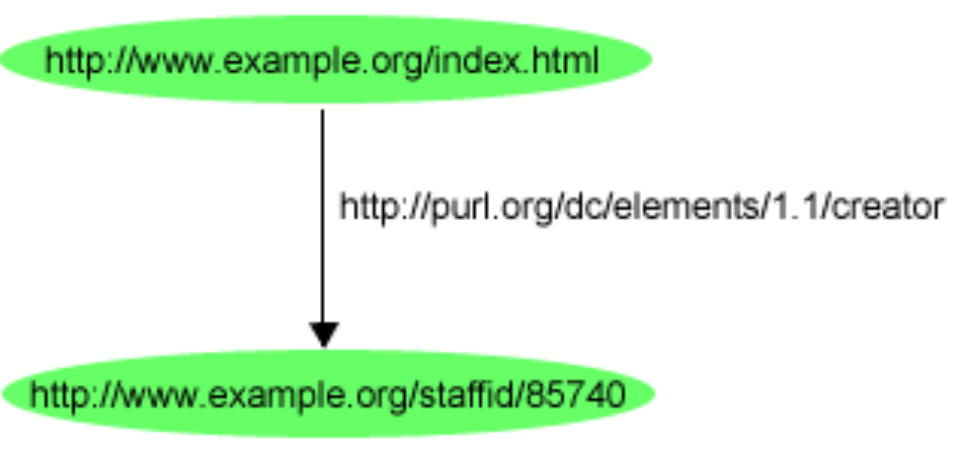
\includegraphics[width=0.4\textwidth]{img/rdf_graph_example.png}
                            \end{center}
                            The graph stands for: 
                            \texttt{http://www.example.org/index.html} has a \texttt{creator} with staff id \texttt{85740}.
                        \end{example}

                    \item[XML] \phantom{}
                        \begin{example} \phantom{}
                            \begin{lstlisting}[mathescape=true, language=xml]
<rdf:RDF
xmlns:rdf=http://www.w3.org/1999/02/22-rdf-syntax-ns#
xmlns:contact=http://www.w3.org/2000/10/swap/pim/contact#>
    <contact:Person rdf:about="http://www.w3.org/People/EM/contact#me">
        <contact:fullName>Eric Miller</contact:fullName>
        <contact:mailbox rdf:resource="mailto:em@w3.org"/>
        <contact:personalTitle>Dr.</contact:personalTitle>
    </contact:Person>
</rdf:RDF>
                            \end{lstlisting}
                        \end{example}
                \end{descriptionlist}

            \item[Database similarities]
                RDF aims to integrate different databases:
                \begin{itemize}
                    \item A DB record is an RDF node.
                    \item The name of a column can be seen as a property type.
                    \item The value of a field corresponds to the value of a property.
                \end{itemize}
        \end{description}

    \item[RDFa] \marginnote{RDFa}
        Specification to integrate XHTML and RDF.

    \item[SPARQL] \marginnote{SPARQL}
        Language to query different data sources that support RDF (natively or through a middleware).

    \item[Ontology web language (OWL)] \marginnote{Ontology web language (OWL)}
        Ontology-based on RDF and description logic fragments.
        Three levels of expressivity are available:
        \begin{itemize}
            \item OWL lite.
            \item OWL DL.
            \item OWL full.
        \end{itemize}

        An OWL has:
        \begin{descriptionlist}
            \item[Classes] Categories.
            \item[Properties] Roles and relations.
            \item[Instances] Individuals.
        \end{descriptionlist}
\end{description}



\section{Knowledge graphs}

\begin{description}
    \item[Knowledge graph] \marginnote{Knowledge graph}
        Knowledge graphs overcome the computational complexity of T-box reasoning with semantic web and description logics.

        \begin{itemize}
            \item Use a simple vocabulary with a simple but robust corpus of types and properties adopted as a standard.
            \item Represent a graph with terms as nodes and edges connecting them.
                Knowledge is therefore represented as triplets \texttt{(h, r, t)} where \texttt{h} and \texttt{t} are entities and \texttt{r} is a relation.
            \item Logic formulas are removed. T-box and A-box can be seen as the same concept. There is no reasoning but only facts.
            \item Data does not have a conceptual schema and can come from different sources with different semantics.
            \item Graph algorithms to traverse the graph and solve queries.
        \end{itemize}

    \item[KG quality] \marginnote{Quality}
        \begin{description}
            \item[Coverage] If the graph has all the required information.
            \item[Correctness] If the information is correct (can be objective or subjective).
            \item[Freshness] If the content is up-to-date.
        \end{description}

    \item[Graph embedding] \marginnote{Graph embedding}
        Project entities and relations into a vectorial space for ML applications.
        \begin{description}
            \item[Link prediction] Given two entities \texttt{h} and \texttt{t}, determine the relation \texttt{r} between them.
            \item[Entity prediction] Given an entity \texttt{h} and a relation \texttt{t}, determine an entity \texttt{t}-related to \texttt{h}.
        \end{description}
\end{description}